% Foliensatz: "AFu-Kurs nach DJ4UF" von DK0TU, Amateurfunkgruppe der TU Berlin
% Lizenz: CC BY-NC-SA 3.0 de (http://creativecommons.org/licenses/by-nc-sa/3.0/de/)
% Autoren: Felix Baum DB4UM <baum@campus.tu-berlin.de>

preamble.dk0tu.tex
\subtitle{Technik A08: \\
           Das elektromagnetische Feld \\[2em]}
\date{Stand 25.5.2015}
 \begin{document}

\begin{frame}
    \titlepage
    \vfill
    \begin{center}
        \ccbyncsaeu\\
        {\tiny This work is licensed under the \em{Creative Commons Attribution-NonCommercial-ShareAlike 3.0 License}.}\\[0.5ex]
         \tiny Amateurfunkgruppe der Technische Universität Berlin (AfuTUB), DKØTU
         %\includegraphics[scale=0.5]{img/DK0TU_Logo.pdf}
    \end{center}
\end{frame}


\section*{Wiederholung}

\begin{frame}
    \frametitle{Wiederholung}
    \begin{center}
		\includegraphics[width=0.7\textwidth]{a08/efeld1.png}\\
		\tiny Abb. 1: elektrisches Feld zwischen zwei leitenden Platten \large
		\begin{itemize}
			\item Was für ein Feld ist dies?
			\item von wo nach wo gehen die Linien?
		\end{itemize}
	\end{center}
\end{frame}

\section*{Elektrisches Feld}

\begin{frame}
    \frametitle{Wie verlaufen die Feldlinien?}
    \begin{center}
        \includegraphics[width=0.8\textwidth]{a08/VFPt_dipole_electric_ohne.png}
        \tiny \hyperlink{refs}{\cite{wm}} \\[1em] \large
    \end{center}
\end{frame}

\begin{frame}
    \frametitle{So verfaufen die Feldlinien}
    \begin{center}
        \includegraphics[width=0.8\textwidth]{a08/VFPt_dipole_electric_mit.png}
        \tiny \hyperlink{refs}{\cite{wm}} \\[1em] \large
    \end{center}
\end{frame}

\begin{frame}
    \frametitle{Elektrisches Feld}
    \begin{center}
        \huge $$E = \frac{U}{d}$$
    \end{center}
\end{frame}

\begin{frame}
    \frametitle{Elektrisches Feld}
    \begin{center}
	\begin{block}{TB512}
        \includegraphics[width=1\textwidth]{a08/TB512.png}\\
        \tiny TB512 \hyperlink{refs}{\cite{bna}}
   		\large Welche elektrische Feldstärke $E$ herrscht in der Mitte der dargestellten, symmetrisch aufgebauten Messzelle, wenn der angeschlossene Sender 1 Watt Ausgangsleistung liefert? 
	\end{block}
    \end{center}
\end{frame}

\begin{frame}
    \frametitle{Elektrisches Feld}
    \begin{center}
	\begin{block}{TB512}
	     \includegraphics[width=1\textwidth]{a08/TB512.png}\\
        \tiny TB512 \hyperlink{refs}{\cite{bna}}\\ \large
		$$U = \sqrt{P \cdot R}$$
		$$E = \frac{U}{d}$$
		$$P = 1W$$
	\end{block}
    \end{center}
\end{frame}

\begin{frame}
    \frametitle{Elektrisches Feld}
    \begin{center}
\begin{block}{TB512}
        \includegraphics[width=1\textwidth]{a08/TB512.png}\\
        \tiny TB512 \hyperlink{refs}{\cite{bna}}
    
    \large $$E = 28.3 \frac{V}{m}$$
\end{block}
    \end{center}
\end{frame}

\begin{frame}
    \frametitle{Starkes Elektrisches Feld}
    \begin{center}
        \includegraphics[width=0.6\textwidth]{a08/Fluorescent_tube_under_electric_line.jpg}
        \tiny \hyperlink{refs}{\cite{wm}} \\[1em] \large
    \end{center}
\end{frame}

\section*{Magnetfeld}

\begin{frame}
    \frametitle{Magnetisches Feld}
    \begin{center}
		\includegraphics[width=0.6\textwidth]{a08/RechteHand.png}\\
		\tiny \hyperlink{refs}{\cite{wm}} \\[1em] \large
		\begin{itemize}
			\item Rechte Hand Regel
			\item Magnetfeld um stromdurchflossenen Leiter
		\end{itemize}
	\end{center}
\end{frame}

\begin{frame}
    \frametitle{Stromdurchflossene Spule}
    \begin{center}
		\includegraphics[width=0.7\textwidth]{a08/H-Feld.png}\\
		\tiny \hyperlink{refs}{\cite{wm}} \\[1em] \large
		\begin{itemize}
		\item Im Inneren ein homogenes Magnetisches Feld
		\item Flussrichtung durch rechte Hand Regel
		\end{itemize}
	\end{center}
\end{frame}

\begin{frame}
    \frametitle{Stromdurchflossene Spule}
    \begin{center}
		\includegraphics[width=0.7\textwidth]{a08/3-D_HFeld.png}\\
		\tiny \hyperlink{refs}{\cite{wm}} \\[1em] \large
		\begin{itemize}
		\item $B = \mu \cdot H$
		\item Im Inneren ein homogenes magnetisches Feld
		\end{itemize}
	\end{center}
\end{frame}

\begin{frame}
    \frametitle{Formeln aus der Formelsammlung}
    \begin{center}
        \huge Leiter: $H = \frac{\mathrm{I}}{l_m}$ \\[1em]
    	\huge Spule: $H = \frac{\mathrm{I} \cdot N}{l_m}$ \\[1em]
    	\huge Spule: $B = \mu_r \cdot \mu_0 \cdot H$\\[1em]
    	 $\mu_0 = 1.257 \cdot 10^{-6}[\frac{Vs}{Am}]$ \\[1em]
    	 $\mu_r = 1$ bei Luft
    \end{center}
\end{frame}

\begin{frame}
    \frametitle{Induktionsofen}
    \begin{center}
		\includegraphics[width=0.56\textwidth]{a08/Induction_heating_of_bar_crop.jpg}\\
		\tiny \hyperlink{refs}{\cite{wm}} \\[1em] \large
		\begin{itemize}
		\item $B = \mu \cdot H$
			\item 15kW bei 450 kHz
			\item Spule ist wassergekühlt
		\end{itemize}
	\end{center}
\end{frame}

\begin{frame}
    \frametitle{Hysterese}
    \begin{columns}[c]
        \column[c]{5cm}
        \begin{center}
        \includegraphics[width=1\textwidth]{a08/Soft_hysteresis_welded.png}\\
        \tiny \hyperlink{refs}{\cite{wm}}
    \end{center}
    \column{5cm} \large
        \begin{center}
        \includegraphics[width=1\textwidth]{a08/Hard_hysteresis_de.png}\\
        \tiny \hyperlink{refs}{\cite{wm}}
    \end{center}
    \end{columns}
\end{frame}

\section*{Elektromagnetisches Feld}
\begin{frame}
    \frametitle{Verständnis Dipol}
    \begin{center}
		\includegraphics[width=1\textwidth]{a08/dipol_entstehung.png}\\
	\end{center}
\end{frame}

\begin{frame}
    \frametitle{Dipol}
    \begin{columns}[c]
        \column[c]{5cm}
        \begin{center}
        \includegraphics[width=1\textwidth]{a08/emagfeld1.png}\\
    \end{center}
    \column{5cm} \large
        \begin{center}
        \includegraphics[width=1\textwidth]{a08/emagfeld2.png}\\
    \end{center}
    \end{columns}
\end{frame}

\section*{Fernfeld}

\begin{frame}
    \frametitle{Polarisation}
    \begin{center}
		\includegraphics[width=1\textwidth]{a08/Onde_electromagnetique.png}\\
		\tiny \hyperlink{refs}{\cite{wm}} \\[1em] \large
		\begin{itemize}
			\item Polarisatzion im Amateurfunk Vertikal oder Horizontal
			\item Elektrisches Feld bestimmt die Polarisation
		\end{itemize}
	\end{center}
\end{frame}

\begin{frame}
    \frametitle{Poynting-Vektor}
    \begin{center}
		\huge $$S = E \times H$$ \\[1em]
		\large Der Poynting-Vektor $S[\frac{W}{m^2}]$ ist das Kreuzprodukt aus dem $E$ und $H$ Feld gibt die Energierichtung, so wie die Wirkleistung des Signals an dem berechneten Punkt.
	\end{center}
\end{frame}

\begin{frame}
    \frametitle{Poynting-Vektor}
    \begin{center}
		\includegraphics[width=1\textwidth]{a08/Poynting_vectors_of_DC_circuit.png}\\
		\tiny \hyperlink{refs}{\cite{wm}} \\[1em] \large
		Rot: E-Feld \\
		Grün: H-Feld
		Blau: Poynting
	\end{center}
\end{frame}

\begin{frame}
    \frametitle{Der Feldwellenwiderstand}
    \begin{center}
        \huge Wie $U = R \cdot \mathrm{I}$  \\[1em]
    	\huge $E = Z_0 \cdot H$ \\[1em]
    	 $Z_0 = \sqrt{\frac{\mu_0}{\epsilon_0}} = 376,7 \Omega $\\[1em]
    \end{center}
\end{frame}

\begin{frame}
    \frametitle{Die Ersatzfeldstärke}
    \begin{center}
        \huge Ersatzfeldstärke des E-Feldes im Fernfeld \\[1em]
    	$E = \frac{1}{r} \sqrt{\frac{Z_0}{4 \cdot \pi} \cdot P_s}$ \\[1em]
    	Es gilt im Freiraum $Z_0 = 376,7 \Omega $\\[1em]
    	$E = \frac{\sqrt{30 \Omega \cdot P_s}}{r} $ \\[1em]
    \end{center}
\end{frame}

\begin{frame}
    \begin{center}
        \Huge Pause
    \end{center}
\end{frame}

\begin{frame}
    \frametitle{Wellenlänge}
    \begin{center}
        \huge Wie lautet die Formel zum Umrechnen von Frequenz auf Wellenlänge?
    \end{center}
\end{frame}

\begin{frame}
    \frametitle{Wellenlänge}
    \begin{center}
        \huge $\lambda = \frac{300}{f}$ mit $f$ in $MHz$
    \end{center}
\end{frame}

\section*{Ionisationsschichten}

\begin{frame}
    \frametitle{Raumwelle}
	\begin{center}
        \includegraphics[width=.9\textwidth]{a08/schichten_behelf_43.png}
        \footnote{\tiny Amateurfunkbehelf s.43 \url{http://ham.granjow.net/builds/Amateurfunkbehelf.pdf}}
    \end{center}
\end{frame}

\begin{frame}
    \frametitle{D-Schicht}
    \begin{itemize}
    			\item Tagsüber und verschwindet nach Sonnenuntergang sehr schnell
				\item Dämpft Frequenzen unter $5MHz$ (160m und 80m unbenutzbar)
       		 	\item HF Frequenzen ab ca $20MHz$ sind bei einem Minimum nicht verwendbar
       		 	\item Bei hoher Sonnenaktivität Möbel-Dellinger-Effekt (Kurzzeitig ganzes KW-Band unbenutzbar)
    \end{itemize}
    \begin{center}
        \includegraphics[width=.6\textwidth]{a08/schichten_behelf_43.png}
        \footnote{\tiny Amateurfunkbehelf s.43 \url{http://ham.granjow.net/builds/Amateurfunkbehelf.pdf}}
    \end{center}
\end{frame}

\begin{frame}
    \frametitle{E-Schicht}
    \begin{itemize}
    			\item Tagsüber
				\item Reflektiert HF-Bänder 10m, 6m
       		 	\item Refelktiert gelegendlich 2m (Sporedic-E) \footnote{\tiny \url{https://www.youtube.com/watch?v=xSWTkuSekhE}}
       		 	\item (Short Skip)mit sehr starken Signalen zwischen 750 und 2200 km (Short-Skip)
    \end{itemize}
    \begin{center}
        \includegraphics[width=.75\textwidth]{a08/schichten_behelf_43.png}
        \footnote{\tiny Amateurfunkbehelf s.43 \url{http://ham.granjow.net/builds/Amateurfunkbehelf.pdf}}
    \end{center}
\end{frame}

\begin{frame}
    \frametitle{F-Schichten}
    \begin{itemize}
    			\item F1 und F2 Schicht
				\item F2 Schicht besteht auch Nachts (langsame Rekombination)
       		 	\item Wichtigstens da beständigste Schichten für KW
       		 	\item (Short Skip)mit sehr starken Signalen zwischen 750 und 2200 km (Short-Skip)
    \end{itemize}
	\begin{center}
        \includegraphics[width=.75\textwidth]{a08/schichten_behelf_43.png}
        \footnote{\tiny Amateurfunkbehelf s.43 \url{http://ham.granjow.net/builds/Amateurfunkbehelf.pdf}}
    \end{center}
\end{frame}

\section*{Besondere Effekte}

\begin{frame}
    \frametitle{Solarer Flux}
    \begin{itemize}
    			\item Messwert der Solaren Radiostrahlung bei $2800 MHz$
				\item Werte über 100 stehen für große Ionisation und somit gute Fernausbreitung von KW
    \end{itemize}
    \begin{center}
        \includegraphics[width=.6\textwidth]{a08/Solar_10_7_cm_Radio_Flux.png}
    \end{center}
\end{frame}

\begin{frame}
    \frametitle{Muf}
        \begin{center}
    \begin{itemize}
    			\item $MUF$: Größte noch nutzbare Frequenz für Reflektion
    			\item $MUF \approx \frac{f_{kritisch}}{sin{\alpha}} = \frac{f_{kritisch}}{cos{\phi}}$
				\item $\alpha$ ist der Astrahlwinkel vom Boden
				\item $\phi$ ist der auftreffwinkel auf die Schicht
				\item $f_{opt} = 0.85 \cdot f_{kritisch}$
    \end{itemize}
        \includegraphics[width=.6\textwidth]{a08/DifferentFrequencies-NPS.png}
    \end{center}
\end{frame}

\begin{frame}
    \frametitle{Fading, Backscatter}
        \begin{center}
    \begin{itemize}
    			\item Von Fading spricht man wenn aufgrund von unterschiedlich starker Ionisierung der Schichten das Signal mal stärker und mal schwächer zu empfangen ist während eines Durchgangs
    			\item Backscatter bezeichnet die Rückstreuung von Wellen und kann bei Frequeznen Weit über der Muf auftreten wenn die Ionosphäre inhomogen ist  			
    			\item \url{https://upload.wikimedia.org/wikipedia/commons/c/c6/Radaroperation.gif}
    			\item Wird bei Radaren genutzt
    \end{itemize}
    \end{center}
\end{frame}

\begin{frame}
    \frametitle{Mögel-Dellinger}
    \begin{center}
    \begin{itemize}
    			\item Entdeckt wurde der Effekt um das Jahr 1930 von Hans Mögel, 1935 hat ihn der John Howard Dellinger dem US-Standardisierungsamt (National Bureau of Standards) vorgestellt.
    			\item Durch Sonneneruptionen, sogenannten Flares, werden Kurzzeitig alle Frequenzen unterhalb von $300MHz$ stark gedämpft durch Ionisierung der D-Schicht
    			\item Im Bild ist Blau Normal und Rot nach dem Flare. \\[1em]
    \end{itemize}
        \includegraphics[width=.6\textwidth]{a08/FlareNPS.png}
    \end{center}
\end{frame}

\begin{frame}
        \begin{center}
        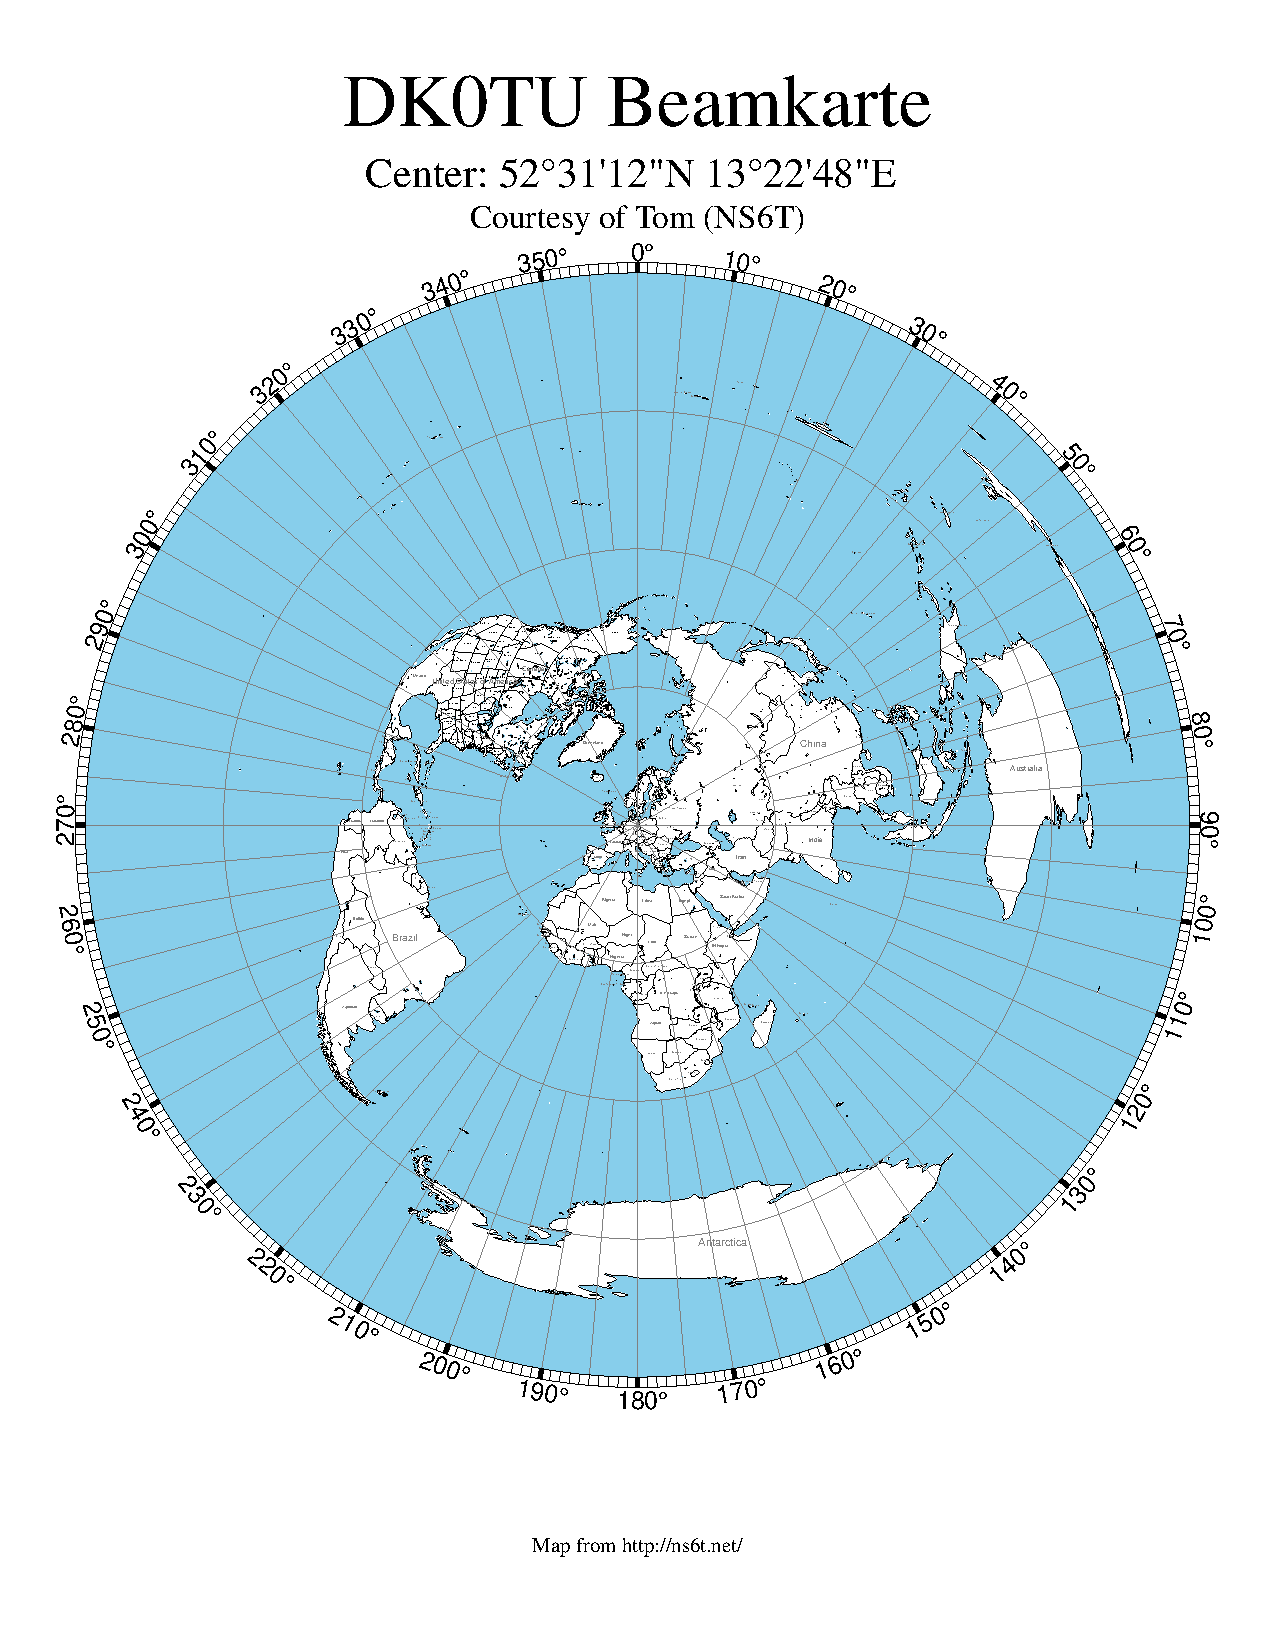
\includegraphics[height=1.2\textheight]{a08/AzimuthalMap.pdf}
    \end{center}
\end{frame}

\begin{frame}
    \frametitle{Reichweite der Bänder}
    \begin{center}
    \begin{itemize}
    			\item Welche Bänder Tagsüber?
    			\item Welche Bänder Nachts?
    			\item Womit geht mehr DX?
    			\item \url{http://www.dr1a.com/pages/de/dx-propagation.php}
    			\item Ausführlich auch in E-Technik e09
    \end{itemize}
    \end{center}
\end{frame}

\renewcommand{\refname}{Referenzen}

\hypertarget{refs}{}
\textcolor{white}{} \\ %\vspace{} geht nicht
\Large Referenzen/Links
\footnotesize

\begin{thebibliography}{}
    \bibitem{darc}  DARC Online-Lehrgang Lektion A08:
                    \url{http://www.darc.de/referate/ajw/ausbildung/darc-online-lehrgang/technik-klasse-a/technik-a08/}
    \bibitem{wm} 	Wikimedia:
                    \url{https://commons.wikimedia.org/wiki/File:VFPt_dipole_electric.svg}
                    \url{https://de.wikipedia.org/wiki/Datei:Fluorescent_tube_under_electric_line.jpg}
                    \url{https://commons.wikimedia.org/wiki/File:RechteHand.png}
                    \url{https://commons.wikimedia.org/wiki/File:Solenoid.png}
                    \url{https://commons.wikimedia.org/wiki/File:VFPt_Solenoid_correct2.svg}
                    \url{https://de.wikipedia.org/wiki/Datei:Induction_heating_of_bar_crop.jpg}
                    \url{https://de.wikipedia.org/wiki/Datei:Soft_hysteresis_welded.svg}
                    \url{https://commons.wikimedia.org/wiki/File:Onde_electromagnetique.svg}
                    \url{https://commons.wikimedia.org/wiki/File:Poynting_vectors_of_DC_circuit.svg}
                    \url{https://commons.wikimedia.org/wiki/File:FlareNPS.gif}
                    \url{}
                    \url{}
                    \url{}
                    \url{}
    \bibitem{beam}  Beamkarten Generator von NS6T:
                    \url{http://ns6t.net/azimuth/azimuth.html}
    \bibitem{wp}    Wikipedia - Die freie Enzyklopädie:
                    \url{https://de.wikipedia.org/wiki/Elektrisches_Feld}
	\bibitem{bna}   Fragenkatalog Bundesnetzargentur Technik Klasse A:                   
                    \url{https://www.bundesnetzagentur.de/SharedDocs/Downloads/DE/Sachgebiete/Telekommunikation/Unternehmen_Institutionen/Frequenzen/Amateurfunk/Fragenkatalog/TechnikFragenkatalogKlasseAf252rId9014pdf.pdf?__blob=publicationFile&v=3}
\end{thebibliography} 

% Hier könnte noch eine Kontaktfolie stehen

\end{document}

